\begin{frame}{Reflections}
    \begin{columns}
        \column{0.4\textwidth}
        $$
            \mathbf{p} =
            x\textcolor{red}{\mathbf{e}_x} +
            y\textcolor{green}{\mathbf{e}_y} +
            z\textcolor{blue}{\mathbf{e}_z} +
            w\textcolor{gray}{\mathbf{e}_0}
        $$

        $$
            \textcolor{gray}{\mathbf{L}} =
            \textcolor{gray}{\mathbf{p}_1} \wedge \textcolor{gray}{\mathbf{p}_2}
        $$

        $$
            \textcolor{u}{\mathbf{p}}_{\textcolor{gray}{\mathbf{L}}} =
            \textcolor{gray}{\mathbf{L}}\, \textcolor{u}{\mathbf{p}_3} \,\textcolor{gray}{\mathbf{L}}^{-1}
        $$

        \column{0.5\textwidth}
        \begin{center}
            \begin{tikzpicture}
                \useasboundingbox (-2,-1) rectangle (2,1);

                \filldraw[gray] (-1.5, -0.643) circle (2pt) node[above left, scale=0.8] {$\mathbf{p}_1$};
                \filldraw[gray] (1.5, 0.643) circle (2pt) node[above left, scale=0.8] {$\mathbf{p}_2$};

                \filldraw[u] (-0.2, 0.5) circle (2pt) node[above left, scale=0.8] {$\mathbf{p}_3$};
                \filldraw[u] (0.35, -0.45) circle (2pt)node[below right, scale=0.8] {$\textcolor{u}{\mathbf{p}}_{\textcolor{gray}{\mathbf{L}}}$};


                \begin{scope}[on background layer]
                    \def\xa{3.5}
                    \def\ya{1.5}
                    \def\scaleFactor{5}
                    \draw[ultra thick, gray, overlay] ({-\scaleFactor*\xa}, {- \scaleFactor*\ya}) -- ({\scaleFactor*\xa}, {\scaleFactor*\ya});
                \end{scope}


                % \draw[red] (current bounding box.south west) rectangle (current bounding box.north east);
            \end{tikzpicture}
        \end{center}

    \end{columns}
\end{frame}

\begin{frame}{What about 2 reflexions?}
    \begin{columns}
        \column{0.4\textwidth}
        $$
            \mathbf{p} =
            x\textcolor{red}{\mathbf{e}_x} +
            y\textcolor{green}{\mathbf{e}_y} +
            z\textcolor{blue}{\mathbf{e}_z} +
            w\textcolor{gray}{\mathbf{e}_0}
        $$

        $$
            \textcolor{gray}{\mathbf{L}_1} \quad
            \textcolor{brokengrey}{\mathbf{L}_2}
        $$

        $$
            \textcolor{u}{\mathbf{p}}_{\textcolor{brokengrey}{\mathbf{L}}} =
            \textcolor{brokengrey}{\mathbf{L}}\, \textcolor{u}{\mathbf{p}} \,\textcolor{brokengrey}{\mathbf{L}}^{-1}
        $$

        $$
            \textcolor{u}{\mathbf{p}}_{\textcolor{brokengrey}{\mathbf{L}} \textcolor{gray}{\mathbf{L}}} =
            \textcolor{gray}{\mathbf{L}}\, \textcolor{u}{\mathbf{p}}_{\textcolor{brokengrey}{\mathbf{L}}}  \,\textcolor{gray}{\mathbf{L}}^{-1}
        $$

        \column{0.5\textwidth}
        \begin{center}
            \begin{tikzpicture}
                \useasboundingbox (-2,-1) rectangle (2,1);

                % \filldraw[gray] (-1.5, -0.643) circle (2pt) node[above left, scale=0.8] {$\mathbf{p}_1$};
                % \filldraw[gray] (1.5, 0.643) circle (2pt) node[above left, scale=0.8] {$\mathbf{p}_2$};

                \filldraw[u] (-0.2, 0.7) circle (2pt) node[above left, scale=0.8] {$\mathbf{p}$};
                \filldraw[u] (0.60, 0.5) circle (2pt)node[above right, scale=0.8] {$\textcolor{u}{\mathbf{p}}_{\textcolor{brokengrey}{\mathbf{L}}}$};
                \filldraw[u] (0.85, 0.1) circle (2pt)node[below right, scale=0.8] {$\textcolor{u}{\mathbf{p}}_{\textcolor{brokengrey}{\mathbf{L}} \textcolor{gray}{\mathbf{L}}}$};

                \begin{scope}[on background layer]
                    \def\xa{3.5}
                    \def\ya{1.5}
                    \def\scaleFactor{5}
                    \draw[ultra thick, gray, overlay] ({-\scaleFactor*\xa}, {- \scaleFactor*\ya}) -- ({\scaleFactor*\xa}, {\scaleFactor*\ya});
                \end{scope}

                \begin{scope}[on background layer]
                    \def\xa{0.5}
                    \def\ya{1.5}
                    \def\scaleFactor{5}
                    \draw[ultra thick, brokengrey, overlay] ({-\scaleFactor*\xa}, {- \scaleFactor*\ya}) -- ({\scaleFactor*\xa}, {\scaleFactor*\ya});
                \end{scope}

                % \draw[red] (current bounding box.south west) rectangle (current bounding box.north east);
            \end{tikzpicture}
        \end{center}

    \end{columns}
    \hfill\href{https://enkimute.github.io/ganja.js/examples/coffeeshop.html\#yYimFv544&fullscreen}{\beamergotobutton{2D rotation}}
\end{frame}


\begin{frame}{Rotation}
    \centering
    \huge
    ... and what if reflecting lines are parallel? \\
    \hfill\href{https://enkimute.github.io/ganja.js/examples/coffeeshop.html\#yYimFv544&fullscreen}{\beamergotobutton{2D rotation}}
\end{frame}




\begin{frame}{But in 3D?}
    \centering
    \huge
    \only<1>{It's the same, with planes!}
\end{frame}


%%%%%%%%%%%%%%%%%%%
\begin{frame}{Interpretation}
    \begin{center}
        \begin{tikzpicture}
            \useasboundingbox (-2,-1) rectangle (2,1);

            % \filldraw[gray] (-1.5, -0.643) circle (2pt) node[above left, scale=0.8] {$\mathbf{p}_1$};
            % \filldraw[gray] (1.5, 0.643) circle (2pt) node[above left, scale=0.8] {$\mathbf{p}_2$};

            \filldraw[u] (-0.2, 0.7) circle (2pt) node[above left, scale=0.8] {$\mathbf{p}$};
            \filldraw[u] (0.60, 0.5) circle (2pt)node[above right, scale=0.8] {$\textcolor{u}{\mathbf{p}}_{\textcolor{brokengrey}{\mathbf{L}}}$};
            \filldraw[u] (0.85, 0.1) circle (2pt)node[below right, scale=0.8] {$\textcolor{u}{\mathbf{p}}_{\textcolor{brokengrey}{\mathbf{L}} \textcolor{gray}{\mathbf{L}}}$};

            \begin{scope}[on background layer]
                \def\xa{3.5}
                \def\ya{1.5}
                \def\scaleFactor{5}
                \draw[ultra thick, gray, overlay] ({-\scaleFactor*\xa}, {- \scaleFactor*\ya}) -- ({\scaleFactor*\xa}, {\scaleFactor*\ya});
            \end{scope}

            \begin{scope}[on background layer]
                \def\xa{0.5}
                \def\ya{1.5}
                \def\scaleFactor{5}
                \draw[ultra thick, brokengrey, overlay] ({-\scaleFactor*\xa}, {- \scaleFactor*\ya}) -- ({\scaleFactor*\xa}, {\scaleFactor*\ya});
            \end{scope}

            % \draw[red] (current bounding box.south west) rectangle (current bounding box.north east);
        \end{tikzpicture}
        \begin{tikzpicture}
            % planes
            \begin{scope}[on background layer, overlay]
                \draw[brokengrey, ultra thick] (0,-50)-- (0,50);
                \draw[gray, ultra thick] (2,-50) -- (2,50);
            \end{scope}
            % intial points
            \filldraw[u] (-0.5,0.5) circle (2pt);
            \filldraw[v]  (-3,-0.5) circle (2pt);
            % second reflexion
            \filldraw[u] (3.5,0.5) circle (2pt);
            \filldraw[v]  (1,-0.5) circle (2pt);
            % line
            \draw[gray,thick,->,>=latex] (-0.5,0.5) -- node[midway,above,black]{$2\mathbf{d}$} (3.5,0.5);
            \draw[gray,thick,->,>=latex] (-3,-0.5)  -- node[midway,above,black]{$2\mathbf{d}$} (1,-0.5);
            %translation
            \draw[gray,thick,->,>=latex] (0,-0.8) -- node[midway,below,black]{$\mathbf{d}$} (2,-0.8);
            % clip
            \clip (-4,1) rectangle (4,1);
        \end{tikzpicture}
    \end{center}
    \Large
    \begin{itemize}
        \item Two successive reflections $\leftrightarrow$ rotation or translation \\
              $\hookrightarrow$ rigid transformation
        \item Quaternions / dual quaternions: 3D cases of motors
        \item Motors (double reflection) work in any dimension!
    \end{itemize}
\end{frame}



%%%%%%%%%%%%%%%%%%
\begin{frame}{Reflexions are generic}
    $$ \mathbf{a}\Big( \textcolor{red}{\mathbf{x}} \wedge \textcolor{green}{\mathbf{y}} \wedge  ... \wedge \textcolor{blue}{\mathbf{z}} \Big) \mathbf{a}^{-1}
        = (\mathbf{a}\textcolor{red}{\mathbf{x}} \mathbf{a}^{-1}) \wedge (\mathbf{a}\textcolor{green}{\mathbf{y}} \mathbf{a}^{-1}) \wedge  ... \wedge  (\mathbf{a}\textcolor{blue}{\mathbf{z}} \mathbf{a}^{-1})$$
    ~\\
    \textbf{Same versor for any object:}
    $$
        \mathbf{a}
        \left\lbrace
        \begin{array}{c}
            \text{point}                  \\
            \textcolor{gray}{line}        \\
            \textcolor{brokengrey}{plane} \\
            \vdots
        \end{array}
        \right\rbrace
        \mathbf{a}^{-1}
    $$
\end{frame}



%%%%%%%%%%%%%%%%
\begin{frame}{Demo in Python}
    \begin{center}
        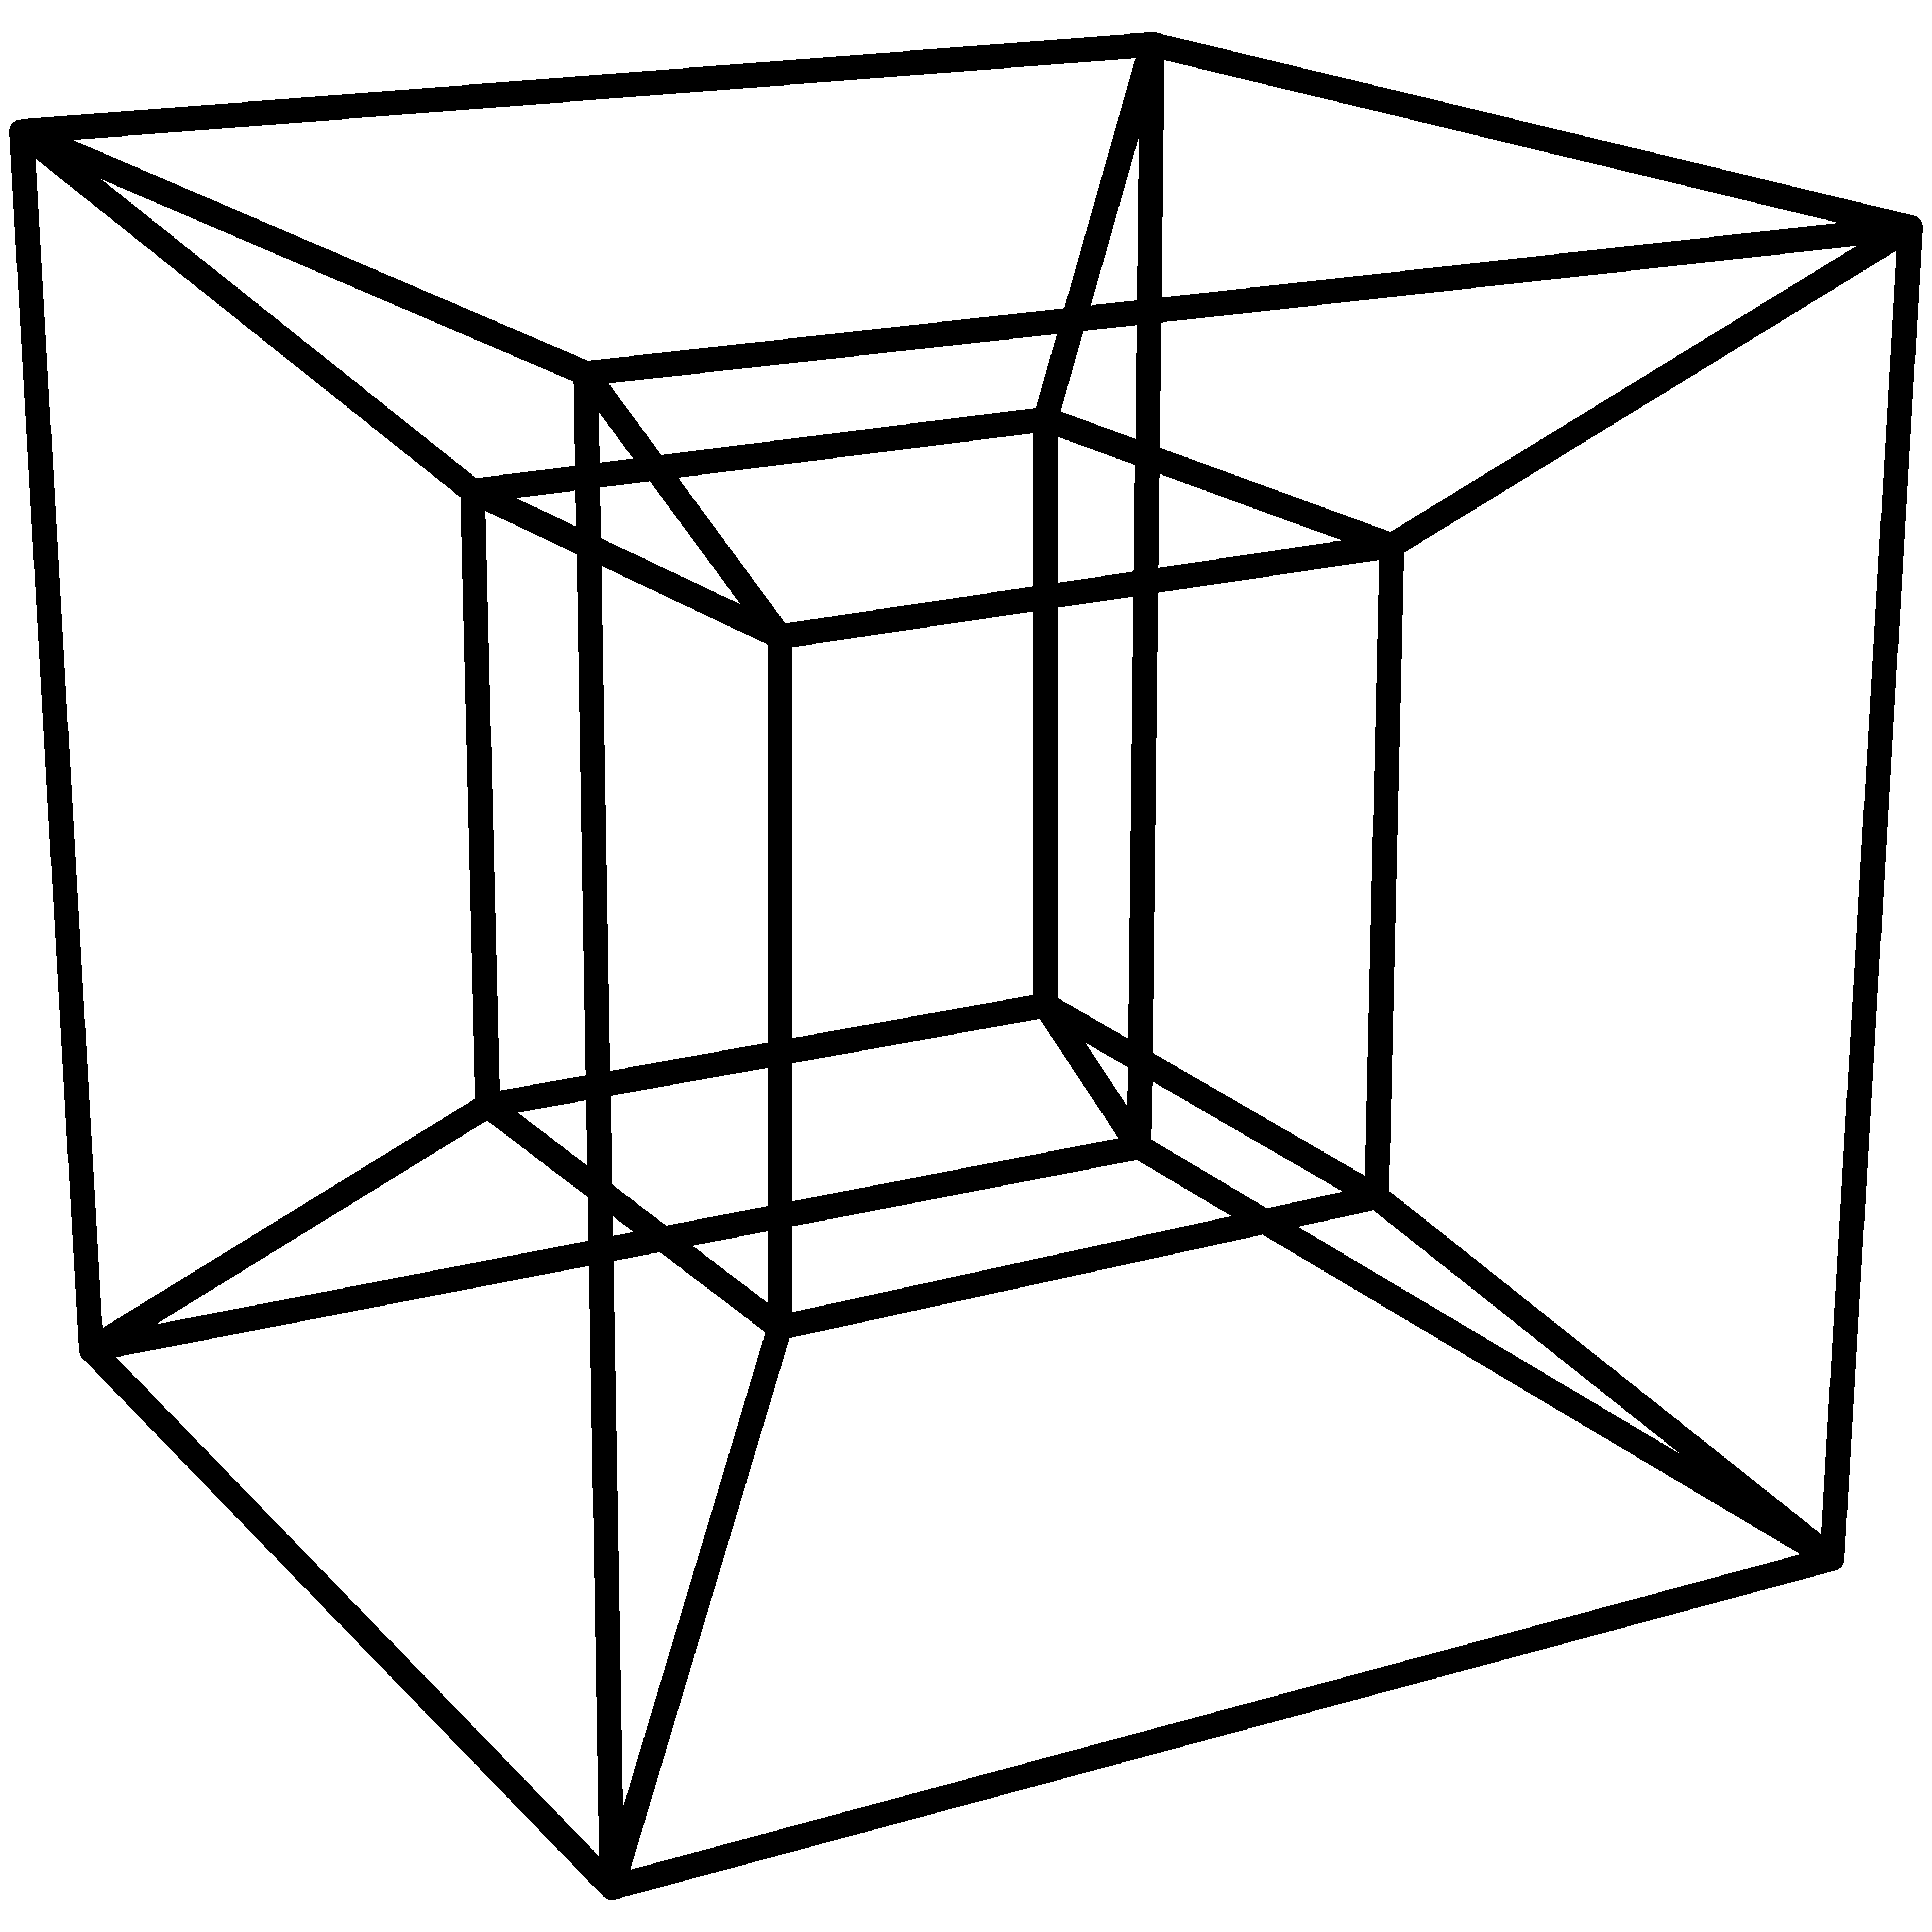
\includegraphics[width=0.4\textwidth]{figures/Tesseract_Mark.pdf}
    \end{center}

    With Kingdon, a Python library for Geometric Algebra made by Martin Roelfs.

    \hfill\href{https://tbuli.github.io/teahouse/lab/index.html}{\beamergotobutton{Hypercube on a string}}

\end{frame}


{\setbeamercolor{palette primary}{fg=black, bg=yellow}
\begin{frame}[standout]
    Questions?
\end{frame}
}



\end{document}


